\chapter{Models}
\label{newmodel}

The files associated with the UAV models used in ProVANT Simulator are located in the following path:

\begin{bashcode}
	$HOME/catkin_ws/src/provant_simulator/source/Database/simulation_elements/models/real
\end{bashcode}

Each model in the simulation environment has a directory with its respective name. This directory contains files that describe the dyanmic, visual, collision and sensorial models, and the control law used. Thus, in case it's necessary to add a new model, or edit an existing one, it must have the UAV's configuration/description files organized as depicted in Figure \ref{modeloorg}.\\

\begin{figure}[H]
	\centering \tt
	\begin{tikzpicture}[%
		grow via three points={one child at (0.5,-0.7) and
			two children at (0.5,-0.7) and (0.5,-1.4)},
		edge from parent path={(\tikzparentnode.south) |- (\tikzchildnode.west)}]
		\node {nome\_do\_modelo/}
		child { node {config/}
			child { node {config.xml}}
		}
		child [missing] {}
		child { node {meshes/}
			child {node {$\star$.stl}}
		}
		child [missing] {}
		child { node {robot/}
			child { node {model.sdf}}
		}
		child [missing] {}
		child { node {model.config}}
		child { node {imagem.gif}};
	\end{tikzpicture}
	\caption{Directory's organization with UAV model description files}
	\label{modeloorg}
\end{figure}

where:

\begin{enumerate}
	\item File \verb config.xml  stores the information regarding the controller to be used in the model.
	\item File \verb model.config  describes thte UAV's dynamic, collision and visual models for simulator Gazebo.
	\item File \verb model.config  describes the model's metadata.
	\item File \verb imagem.gif  contains the image used by the garphical interface to illustrate the UAV model (see Figure \ref{tela_inicial.jpg}, item 2).
	\item The directory \verb meshes  stores the files exported from the CAD tool (used for the UAV's mechanical design), like SolidWorks.
\end{enumerate}

The file \verb model.config  tells Gazebo where is the file with the model's strucutal data and provides information regarding the models's author, version and description. Figure \ref{model.config} illustrates an example of this file. The tags used in \verb model.config  are:

\small
\begin{itemize}
	\setlength{\itemsep}{1pt}
	\setlength{\parskip}{0pt}
	\setlength{\parsep}{0pt}
	\xmlfield{name}{The model's name}
	\xmlfield{version}{The model's version}
	\xmlfield{sdf}{Path to the file that describes the Gazebo model's dynamic, colision and visual characteristics}
	\item[-] \textcolor{blue}{\texttt{<author>}}
	\begin{itemize}
		\xmlfield{name}{The author's name}
		\xmlfield{email}{Author's email adress}
	\end{itemize}
	\textcolor{blue}{\texttt{</author>}}
	\xmlfield{description}{Brief description of the model}
\end{itemize}
\normalsize

\begin{code}[H]
	\begin{minted}[obeytabs=true,tabsize=4]{xml}
		<?xml version="1.0"?>
		<model>
			<name>vant</name>
			<version>1.0</version>
			<sdf version='1.5'>robot/model.sdf</sdf>
			<author>
				<name>provant</name>
				<email>provant@ufmg.br</email>
			</author>
			<description>
				The UAV version 3.0 of the provant project 
			</description>
		</model>
	\end{minted}
	\caption{Example content for file \texttt{model.config}}
	\label{model.config}
\end{code}

The file \verb config.xml  stores all the settings regarding the control structure to be used during the simulation, such as sensors, actuatores, control laws and sampling period. ith the purpose of helping the user to edit this file, the graphical interface provides tools for this task, so that the user won't have to directly access this file. Code \ref{config.xml} illustrates an example of this file:

\begin{code}[H]
	\begin{minted}[obeytabs=true,tabsize=4]{xml}
		<?xml version="1.0" encoding="UTF-8"?>
		<config>
			<TopicoStep>Step</TopicoStep>
			<Sampletime>12</Sampletime>
			<Strategy>libvant3_lqr.so</Strategy>
			<RefPath>ref.txt</RefPath>
			<Outputfile>out.txt</Outputfile>
			<InputPath>in.txt</InputPath>
			<ErroPath>erro.txt</ErroPath>
			<Sensors>
				<Device>Estados</Device>
			</Sensors>
			<Actuators>
				<Device>ThrustR</Device>
				<Device>ThrustL</Device>
				<Device>TauR</Device>
				<Device>TauL</Device>
				<Device>Elevdef</Device>
				<Device>Ruddef</Device>
			</Actuators>
		</config>
	\end{minted}
	\caption{Example of \texttt{config.xml} file}
	\label{config.xml}
\end{code}

The tags used in file \verb config.xml  are:

\small
\begin{itemize}
	\setlength{\itemsep}{1pt}
	\setlength{\parskip}{0pt}
	\setlength{\parsep}{0pt}
	\xmlfield{TopicoStep}{The sincronization topic between the simulator and the controller. \textbf{This tag's value must not be changed.}}
	\xmlfield{Sampletime}{The controller's smapling period, in milliseconds}
	\xmlfield{Strategy}{Name of the library associated to the implementation of the control strategy to be used along with this model}
	\xmlfield{RefPath}{Name of the file where the setpoint signal data is stored}
	\xmlfield{Outputfile}{Name of the file where the control signal data is stored}
	\xmlfield{InputPath}{Name of the file where the sensor data is stored}
	\xmlfield{ErroPath}{Name of the file where the error vector data is stored}
	\xmlfield{Sensors}{Name of the sensor topics to which the control strategy will have access (in the specified order)}
	\xmlfield{Actuators}{Name of the actuator topics to which the control strategy will have access (the controller must return a vector with the same amount of data and in the order specified here)}
\end{itemize}
\normalsize

File \verb model.sdf  provides to Gazebo the UAV model's information in XML format following the \href{http://sdformat.org/spec}{SDF format} (Figure \ref{geral} illustrates an example of this file). The next section describes more thoroughly the basic structure of an SDF file.

\section{The SDF file}

Before presenting the basic configuration of an SDF file, it's necessary to introduce a few concepts.

In the simulator, a model correspond to a mechanical system, which can be formed my one or multiple rigid bodies\footnote{By assuming a body as rigid, the elasticity and deformation effects are neglected}. Thus, as in a manipulator, the bodies in the simulator are called links. Child links are connected to parent links by joints. Child links are rigid bodies whose movements are restricted by the connection (joint) with bodies called parent links. The links have inertial, visual and collision properties.

As for joints, they impose restrictions to the relative movement between two links and have properties such ase joint type (prismatic, revolute, etc.), movement limits (position ans speed), friction, etc. Code \ref{geral} illustrates an example of an SDF file.

\begin{code}[H]
	\begin{minted}[obeytabs=true,tabsize=4]{xml}
		<?xml version="1.0" encoding="UTF-8"?>
		<sdf version="1.4">
			<model name="modelo">
				<link name="corpo">
					...
				</link>
				<link name="servo">
					...
				</link>
				<joint name="corpo_servo">
					...
				</joint>
			</model>
		</sdf>
	\end{minted}
	\caption{Description of a model in file \texttt{model.sdf}}
	\label{geral}
\end{code}

The tags used are:

\small
\begin{itemize}
	\setlength{\itemsep}{1pt}
	\setlength{\parskip}{0pt}
	\setlength{\parsep}{0pt}
	\xmlfield{link}{Describes a link, specifying its name}
	\xmlfield{joint}{Describes a joint, specifying its name}
\end{itemize}\normalsize

Each link in the model has trhee types of description for the simulator: the kinematic, visual and collision descriptions. The configuration structure of a link in an SDF file has athe format depicted in code \ref{elo}:

\begin{code}[H]
	\begin{minted}[obeytabs=true,tabsize=4]{xml}
		<link name="servodir">
			<pose>0.02E-3 -277.61E-3 56.21E-3 -0.0872665 0 0</pose>
			<inertial> 
				...
			</inertial>
			<collision name="servodircollision"> <!--opcional-->
				...
			</collision>
			<visual name="servodirvisual"> <!--opcional-->
				...
			</visual>
		</link>
	\end{minted}
	\caption{Description of a link in file \texttt{model.sdf}}
	\label{elo}
\end{code}

The tags used are:

\small
\begin{itemize}
	\setlength{\itemsep}{1pt}
	\setlength{\parskip}{0pt}
	\setlength{\parsep}{0pt}
	\xmlfield{pose}{Link's pose}
	\xmlfield{inertial}{Link's inertial properties}
	\xmlfield{collision}{Link's collision properties. The collision models for the UAVs used in the simulation environment are obtained from CAD files.}
	\xmlfield{visual}{Visual characteristics such as color and shape. The visual models for the UAVs used in the simulation environment are obtained from CAD files, except for the color, which is specified separately.}
\end{itemize}
\normalsize

\noindent \textbf{Links inertial parameters:} The user must inform each link's inertial parameters inside the tag \verb inertial . The required information are the mass, the center of mass' relative position and the inertia tensor. In Code \ref{inertial} an exemple configuration of a link's inertial parameters in format SDF is illustrated.

\begin{code}[H]
	\begin{minted}[obeytabs=true,tabsize=4]{xml}
		<inertial>
			<mass>0.0809439719362664</mass>
			<pose>
				-3.60859273452335E-10 -0.000226380714807978 0.0594780519701684 0 0 0
			</pose>
			<inertia>
				<ixx>3.88267747087835E-06</ixx>
				<ixy>6.03219085082653E-06</ixy>
				<ixz>-2.78471406661236E-12</ixz>
				<iyy>0.000104858690365283</iyy>
				<iyz>7.0486590219062E-07</iyz>
				<izz>8.31755564684115E-05</izz>		
			</inertia>
		</inertial>
	\end{minted}
	\caption{Description of inertial characteristics in file \texttt{model.sdf}}
	\label{inertial}
\end{code}

The tags used are:

\small
\begin{itemize}
	\setlength{\itemsep}{1pt}
	\setlength{\parskip}{0pt}
	\setlength{\parsep}{0pt}
	\xmlfield{mass}{The link's mass}
	\xmlfield{pose}{The center of mass' position relative to its main coordinate system}
	\xmlfield{inertia}{The link's inertia tensor}
\end{itemize} 
\normalsize

\noindent \textbf{Link's collision properties:} In order for collision effects to be applied to the link, the user must describe the link's shape in file \verb model.sdf . There are many ways to describe it, but this guide presents only the method used in the UAV models in ProVANT Simulator, which consists of importing files created with CAD tools, such as SolidWorks. Code \ref{colision} shows an example descriptioin of a link's visual parameters using an STL file:

\begin{code}[H]
	\begin{minted}[obeytabs=true,tabsize=4]{xml}
		<collision name="servodircollision">
			<pose>0 0 0 0 0 0</pose>
			<geometry>
				<mesh>
					<uri>model://vant_2comcarga/meshes/servodir.STL</uri>
				</mesh>
			</geometry>
		</collision>
	\end{minted}
	\caption{Description of collision characteristics in file \texttt{model.sdf}}
	\label{colision}
\end{code}

The tags used are:

\small
\begin{itemize}
	\setlength{\itemsep}{1pt}
	\setlength{\parskip}{0pt}
	\setlength{\parsep}{0pt}
	\xmlfield{pose}{The collision model's pose relative to the link's coordinates' origin}
	\item[-] \textcolor{blue}{\texttt{<geometry>}}
	\begin{itemize}
		\item[-] \textcolor{blue}{\texttt{<mesh>}}
		\begin{itemize}
			\xmlfield{uri}{Path to the mesh file, relative to the model's directory, obtained by exporting from SolidWorks}
		\end{itemize}
		\textcolor{blue}{\texttt{</mesh>}}
	\end{itemize}
	\textcolor{blue}{\texttt{</geometry>}}
\end{itemize}
\normalsize

\noindent \textbf{Links visual properties:} In order for the link o be visualized during the simulation, the user must describe the link's visual parameters in file \verb model.sdf . Just like in the previous case, there are several description methods, but this guide illustrates only the one used in the simulation environment's UAVs, which consists of importing files created from CAD tools. Code \ref{visual} Shows an example description of a link's visual parameters using an STL file:

\begin{code}[H]
	\begin{minted}[obeytabs=true,tabsize=4]{xml}
		<visual name="servodirvisual">
			<pose>0 0 0 0 0 0</pose>
			<geometry>
				<mesh>
					<uri>model://vant_2comcarga/meshes/servodir.STL</uri>
				</mesh>
			</geometry>
			<material>
				<ambient>0 0 0 0</ambient>
				<diffuse>1 1 1 1</diffuse>
				<specular>0.1 0.1 0.1 1</specular>
				<emissive>0 0 0 0</emissive>
			</material>
		</visual>
	\end{minted}
	\caption{Description of visual characteristics in file \texttt{model.sdf}}
	\label{visual}
\end{code}

The tags used are:

\small
\begin{itemize}
	\setlength{\itemsep}{1pt}
	\setlength{\parskip}{0pt}
	\setlength{\parsep}{0pt}
	\xmlfield{pose}{The visual model's pose relative to the link's coordinates' origin}
	\item[-] \textcolor{blue}{\texttt{<geometry>}}
	\begin{itemize}
		\item[-] \textcolor{blue}{\texttt{<mesh>}}
		\begin{itemize}
			\xmlfield{uri}{Path to the mesh file, relative to the model's directory, obtained by exporting from SolidWorks}
		\end{itemize}
		\textcolor{blue}{\texttt{</mesh>}}
	\end{itemize}
	\textcolor{blue}{\texttt{</geometry>}}
	\item[-] \textcolor{blue}{\texttt{<material>}}
	\begin{itemize}
		\xmlfield{ambient}{Ambient color}
		\xmlfield{diffuse}{Diffuse color}
		\xmlfield{specular}{Specular color}
		\xmlfield{emissive}{Emissive color}
	\end{itemize}
	\textcolor{blue}{\texttt{</material>}}
\end{itemize} 
\normalsize

\subsection{Joint description} 

Ther joint types in the simulator are:

\begin{itemize}
	\item \textbf{revolute}: Rotation movement;
	\item \textbf{gearbox}: Revolute joint with transmission gears between links with different torque and speed ratios;
	\item \textbf{revolute2}: Joint composed by two revolute joints in series;
	\item \textbf{prismatic}: Prismatic joint;
	\item \textbf{universal}: Joint behaving as an articulated sphere;
	\item \textbf{piston}: Joint behaving as a combination of a revolute and a prismatic joint.
\end{itemize}

An example of a joint's configuration structure is shown in Code \ref{joint}.
\begin{code}[H]
	\begin{minted}[obeytabs=true,tabsize=4]{xml}
		<joint name="aR" type="revolute">
			<pose>0 0 0 0 0 0</pose>
			<parent>corpo</parent>
			<child>servodir</child>
			<axis>
				<xyz>0 0.9962 -0.0872</xyz>
				<limit>
					<lower>-1.5</lower>
					<upper>1.5</upper>
					<effort>2</effort>
					<velocity>0.5</velocity>
				</limit>
				<dynamics>
					<damping>0</damping>
					<friction>0</friction>
				</dynamics>
			</axis>
		</joint>
	\end{minted}
	\caption{Joint description in file \texttt{model.sdf}}
	\label{joint}
\end{code}
The tags used are:

\begin{itemize}
	\setlength{\itemsep}{1pt}
	\setlength{\parskip}{0pt}
	\setlength{\parsep}{0pt}
	\xmlfield{pose}{Child link's pose relative to the parent link}
	\xmlfield{parent}{Parent link's name}
	\xmlfield{axis}{Unit vector corresponding to the joint's rotation axis (expressed in the model's coordinate system if the SDF version is 1.4, or in the child link's coordinate system if the version is 1.6)}
	\xmlfield{lower}{Lower limit to the joint's position (in radians if it's a revolute joint or meters if it's prismatic)}
	\xmlfield{upper}{Upper limit to the joint's position (in radians if it's a revolute joint or meters if it's prismatic)}
	\xmlfield{velocity}{Joint's speed limit (in rad/s if it's a revolute joint or m/s if it's prismatic)}
	\xmlfield{effort}{Joint's effort limit (in N$\cdot$m if it's a revolute joint or N if it's prismatic)}
	\xmlfield{damping}{Vicous friction coefficient}
	\xmlfield{friction}{Static friction coefficient}
\end{itemize}

\subsection{Plugin description}
\label{plugins}

Plugins are dynamic libraries loaded during the simulator's initialization, using the configurations stored in the model description file (SDF file). These libraries are used to implement the sensors and actuators in the simulation environment.

ProVANT Simulator only uses two of \href{http://gazebosim.org/tutorials/?tut=plugins_hello_world}{Gazebo's plugin types} for the UAV model's control and monitoring: Model and Sensor.

\noindent \textbf{Model plugins:} Model plugins are dynamic libraries which control and monitor the UAV model's simulation variables. With them it's possible to create customized sensors and actuators. To insert a model plugin in file \verb model.sdf , the user must add \textcolor{blue}{\texttt{<plugin>}} tags defining its name, the dynamic library's name and the internal tags required to configure the plugin. Code \ref{pluginmod} exemplifies the insertion process.

The options for model plugins available in ProVANT Simulator are detailed in appendix \ref{pluginsAp}.

\begin{code}[H]
	\begin{minted}[obeytabs=true,tabsize=4]{xml}
		<?xml version="1.0" encoding="UTF-8"?>
		<sdf version="1.4">
			<model name="modelo">
				<link name="corpo">
					...
				</link>
				<link name="servo">
					...
				</link>
				<joint name="corpo_servo">
					...
				</joint>
				<plugin name="plugin_servo">
					...
				</plugin>
			</model>
		</sdf>
	\end{minted}
	\caption{Insertion of model plugins in file \texttt{model.sdf}}
	\label{pluginmod}
\end{code}

\noindent \textbf{Sensor plugins:} Sensor plugins are dynamic lybraries to simulate sensors, used by ProVANT Simulator to measure data from a UAV model. To insert sensor plugins, the user must add \textcolor{blue}{\texttt{<sensor>}} tags defining its name and the internal tags required to configure the plugin. Code \ref{pluginsen} exemplifies the insertion process.

\begin{code}[t]	
	\begin{minted}[obeytabs=true,tabsize=4]{xml}
		<link name="servodir">
			<pose>0.02E-3 -277.61E-3 56.21E-3 -0.0872665 0 0</pose>
			<inertial> 
				...
			</inertial>
			<collision name="servodircollision"><!--opcional-->
				...
			</collision>
			<visual name="servodirvisual"> <!--opcional-->
				...
			</visual>
			<sensor name="servosensor"> <!--opcional-->
				...
			</sensor>
			<sensor name="servosensor2"> <!--opcional-->
				...
			</sensor>
		</link>
	\end{minted}
	\caption{Insertion of sensor plugins in file \texttt{model.sdf}}
	\label{pluginsen}	
\end{code}

The sensor available in ProVANT Simulator are GPS, IMU, sonar and magnetometer (\href{http://sdformat.org/spec}{more details} on their configuration in file \verb model.sdf ). However, those sensors don't have a communication interface with ROS, since they broadcast their date via Gazebo topics. To broadcast these data to ROS topics the user must add, along with the sensor plugins, model plugins. Such plugins are specified in appendix \ref{pluginsAp}.

Note: In order for the sensor to work properly, the user must adjust the sampling rate to exactly the inverse of the simulation step (e.g. 1000~Hz).

\subsection{Communication messages' standard}

As a standard, all plugins and sensor available in the simulation environment make their provide their data using the same data structure. This data structure is abstracted in ROS through messages. Messages are simple data structures containing typed fields. The sensor plugins' standard message is illustrated below, where:

\begin{itemize}
	\item \verb header : provides the time instant in which the data as obtained, the frame and the sequential ID
	\item \verb name : provides the name of the instrument which provided the message
	\item \verb values : vector containing the data provided by the sensors
\end{itemize} 

\begin{code}[H]
	\begin{verbatim}
		- Header header
		- string name
		- float64[] values
	\end{verbatim}	
\end{code}

The controller, in turn, receives a type of message which stores the messages of all sensors from a given simulation step in the same place and in a user-defined order, as described in section \ref{sensoresatuadores}. This type is illustrated below:

\begin{code}[H]
	\begin{verbatim}
		- Header header
		- string name
		- float64[] values
	\end{verbatim}
\end{code}
\section{UAV Models}

In this chapter section all uav models available in the simulator will be detailed. Each uav will be described showing its state vector, the coordinate frames used to derive the kinematic and dynamic models and a table with parameters.

\subsection{UAV 2.0}

The first model implemented in the simulator was the UAV 2.0. The UAV was implemented with the goal to allow the user to simulate a simple tilt rotor UAV.

\begin{figure*}[!ht]
	\centering
	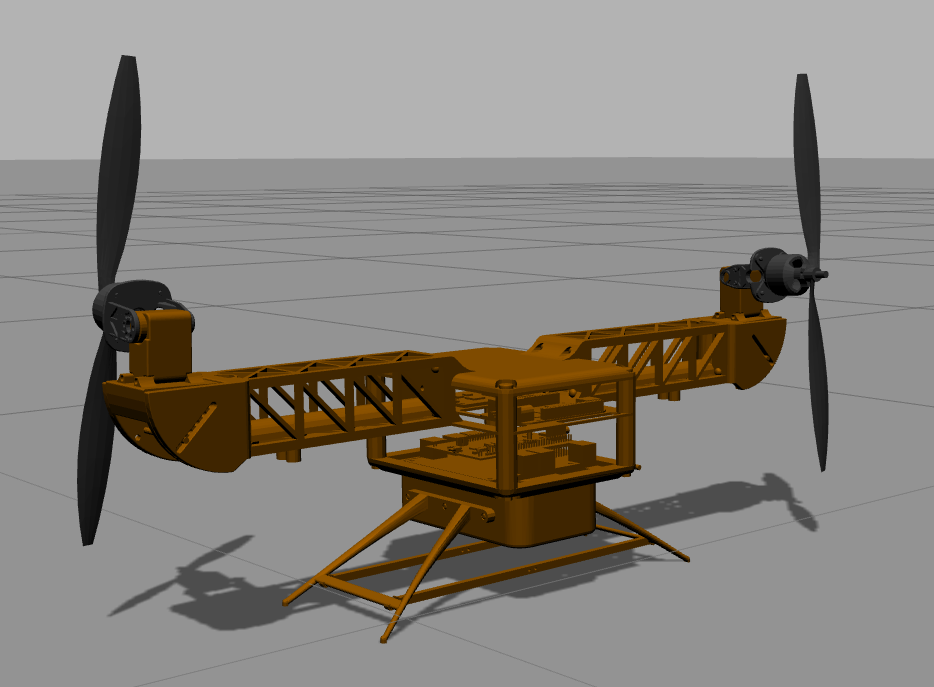
\includegraphics[width=250pt]{figuras/vant2.png}
	\caption{Modelo VANT 2.0 }
	\label{vant2}
\end{figure*}

The kinematic model and dynamic model were developed using the frames displayed in figure \ref{v2frames} and the parameters showned in table \ref{v2_tab} ignoring the terms referent to the load parameters.

\begin{figure} [!ht]
	\centering
	\begin{minipage}{.5\textwidth}
		\centering
		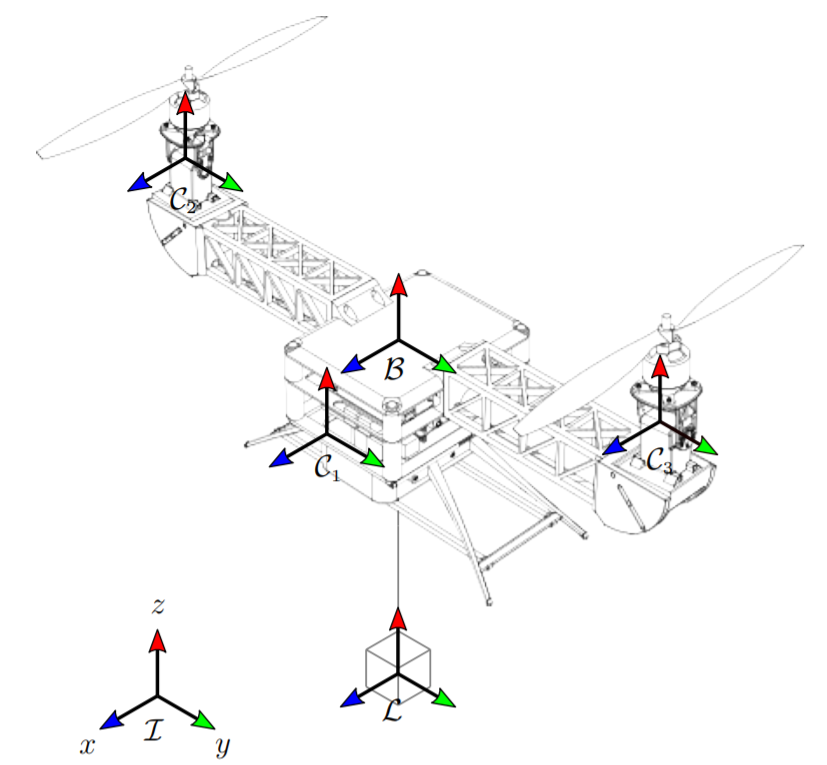
\includegraphics[width=250pt]{figuras/v2loadframes}
		\caption{UAV 2.0  Coordinate Frames}
		\label{v2frames}
	\end{minipage}%
	\begin{minipage}{.5\textwidth}
		\centering
		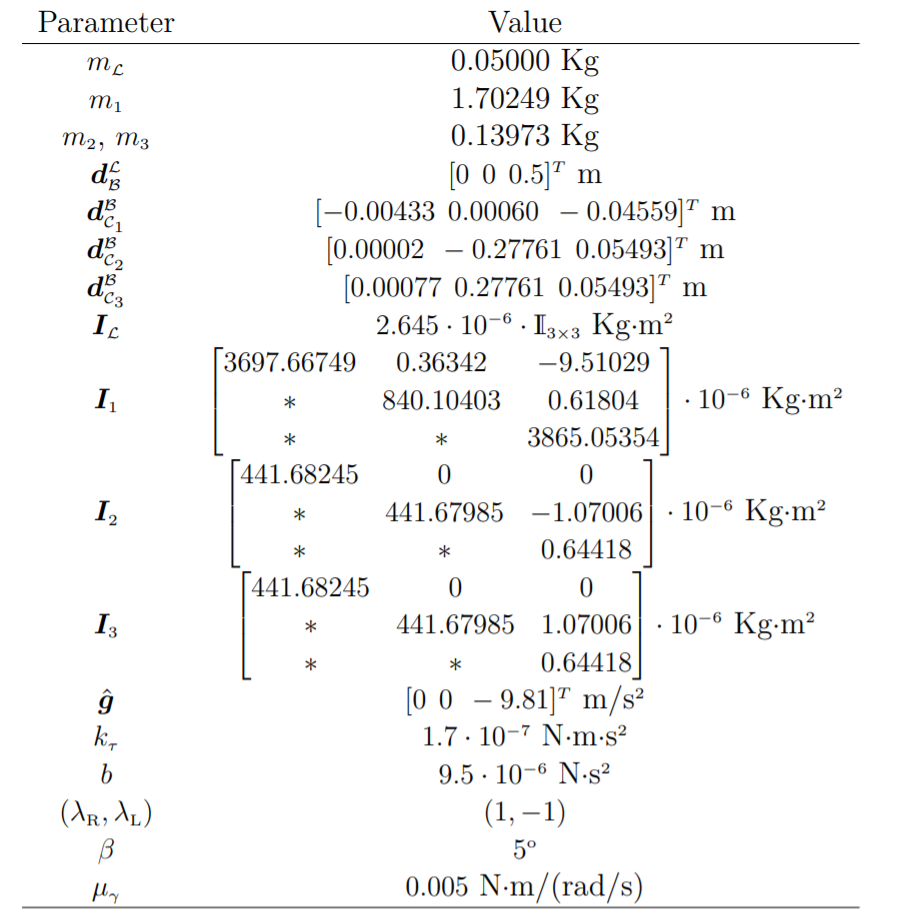
\includegraphics[width=250pt]{figuras/v2loadtab}
		\caption{UAV 2.0 Parameters}
		\label{v2_tab}
	\end{minipage}
\end{figure}

The model was implemented with an LQR control strategy with the followinf state vector:
\begin{equation*}
\bm{X} = \begin{bmatrix}
x & y & z & \phi & \theta & \psi
\end{bmatrix}'
\end{equation*} 

Three plugins were employed in the UAV simulation: The "brushless" plugin to apply the forces generated by the propellers, the "servo" plugin to allow actuate the servo motors, and the "statespace" to access the UAV state vector needed for control. This plugins are further detailed in appendix \ref{pluginsAp}. In figure \ref{v2graph}, the rectangular shapes indicate the ros topics and the roud shapes represent the ros nodes trigger in the simulation.

\begin{figure*}[!ht]
	\centering
	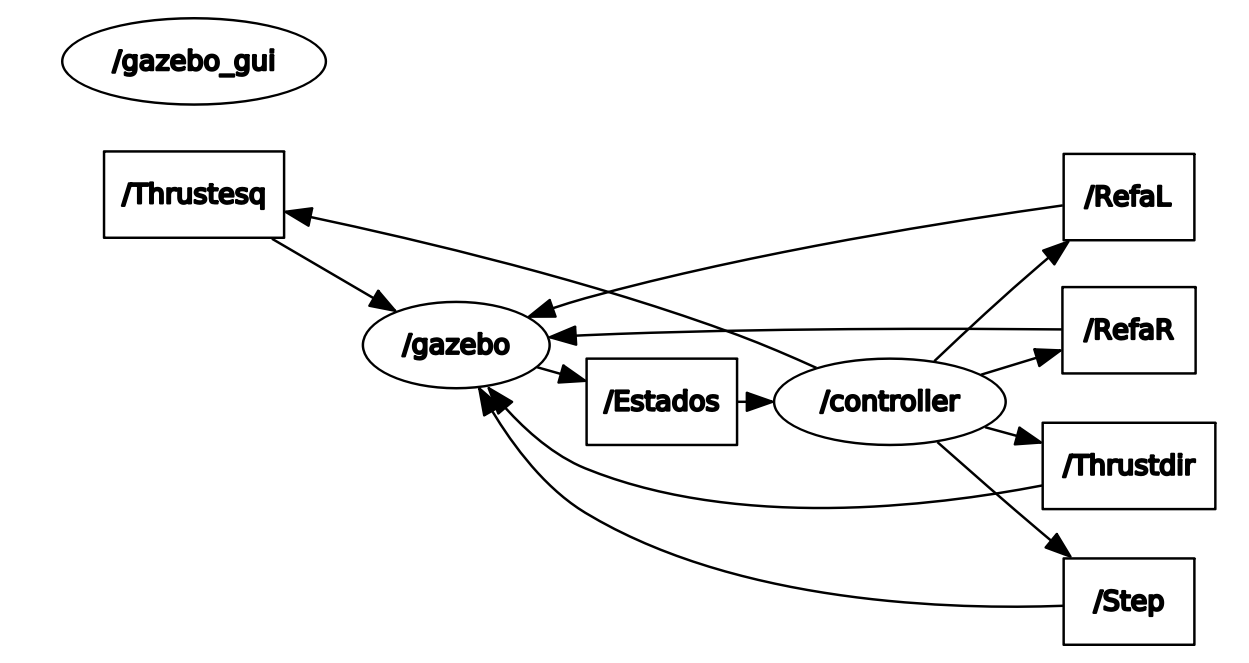
\includegraphics[width=350pt]{figuras/v2graph.png}
	\caption{UAV 2.0 Load Communication}
	\label{v2graph}
\end{figure*}

\subsection{UAV 2.0 Load}


The second model implemented in the simulator was the UAV 2.0 for load transportation missions. The UAV was implemented with the goal to allow the user to simulate a recurrent topic in UAV research, the load transportantion problem. This problem was extensively studied in the ProVANT project and approached in several works like in this paper:\url{https://www.researchgate.net/publication/327836019_Suspended_Load_Path_Tracking_Control_Using_a_Tilt-rotor_UAV_Based_on_Zonotopic_State_Estimation}.

\begin{figure*}[!ht]
	\centering
	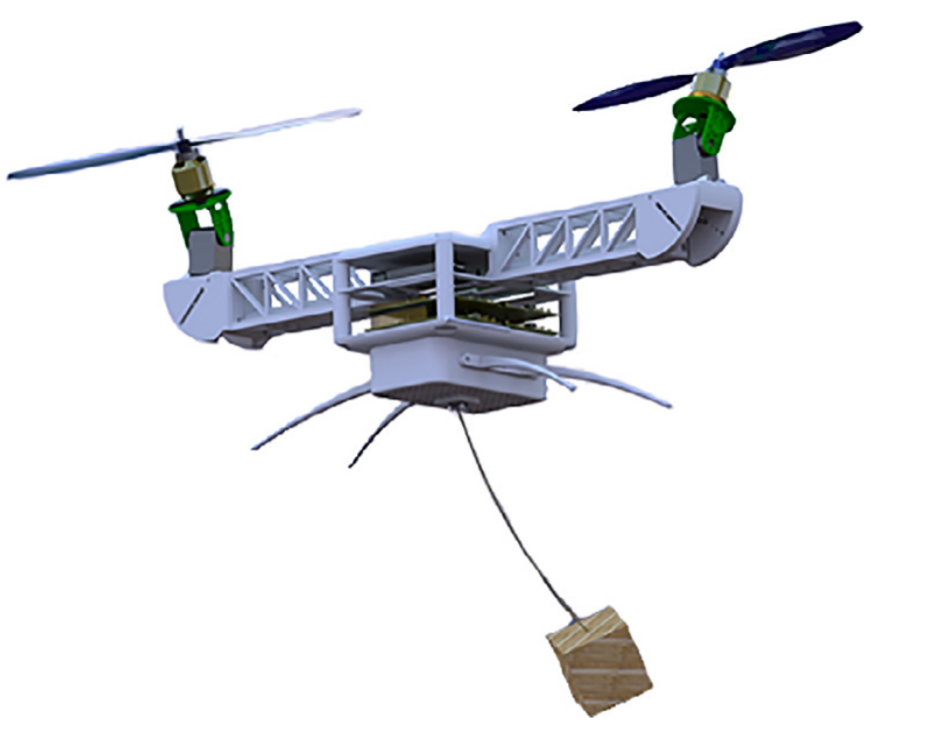
\includegraphics[width=250pt]{figuras/vant2load.png}
	\caption{VANT 2.0 Load}
	\label{vant2load}
\end{figure*}

The kinematic model and dynamic model were developed using the frames displayed in figure \ref{v2loadframes} and the parameters showned in table \ref{v2tab}

\begin{figure} [!ht]
	\centering
	\begin{minipage}{.5\textwidth}
		\centering
		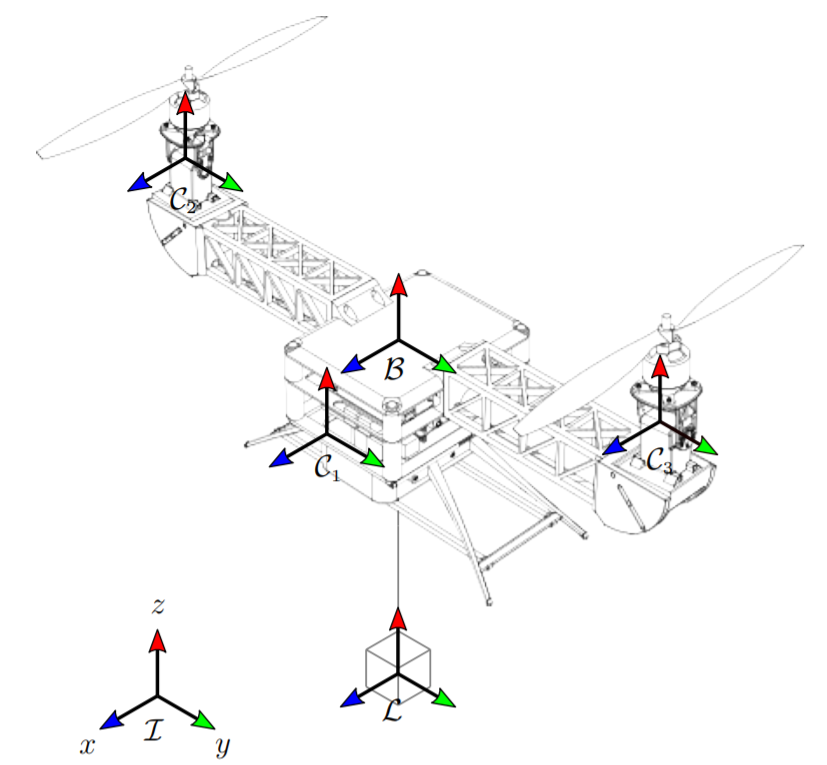
\includegraphics[width=250pt]{figuras/v2loadframes}
		\caption{UAV 2.0 Load Coordinate Frames}
		\label{v2loadframes}
	\end{minipage}%
	\begin{minipage}{.5\textwidth}
		\centering
		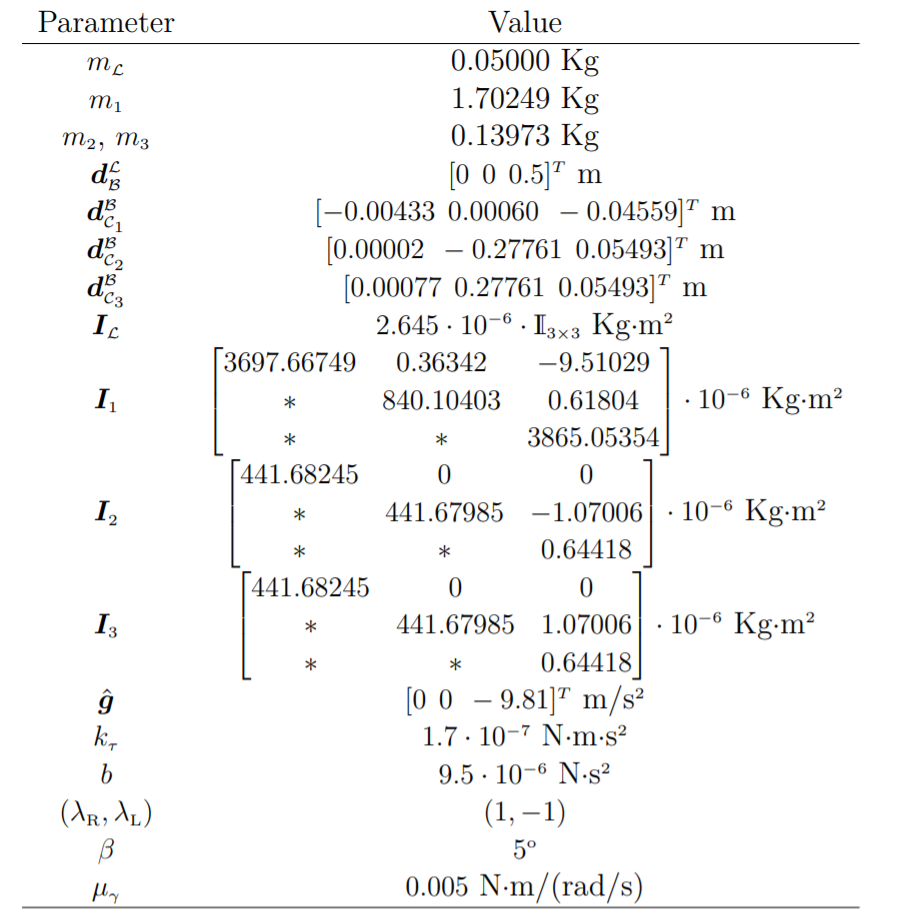
\includegraphics[width=250pt]{figuras/v2loadtab}
		\caption{UAV 2.0 Load Parameters}
		\label{v2tab}
	\end{minipage}
\end{figure}

The model was implemented with an $\mathcal{H}_\infty$ control strategy with the followinf state vector:
\begin{equation*}
\bm{X} = \begin{bmatrix}
\bm{q} & \bm{\dot{q}} & \int{x} & \int{y} & \int{z} & \int{\psi}
\end{bmatrix}'
\end{equation*} 

Where, 
\begin{equation*}
\bm{q} = \begin{bmatrix}
x & y & z & \phi & \theta & \psi & x_{load} & y_{load} & \alpha_R & \alpha_L
\end{bmatrix}' 
\end{equation*} 

Three plugins were employed in the UAV simulation: The "brushless" plugin to apply the forces generated by the propellers, the "servo" plugin to allow actuate the servo motors, and the "statespaceload" to access the UAV state vector needed for control. This plugins are further detailed in appendix \ref{pluginsAp}. In figure \ref{v2loadgraph}, the rectangular shapes indicate the ros topics and the roud shapes represent the ros nodes trigger in the simulation.

\begin{figure*}[!ht]
	\centering
	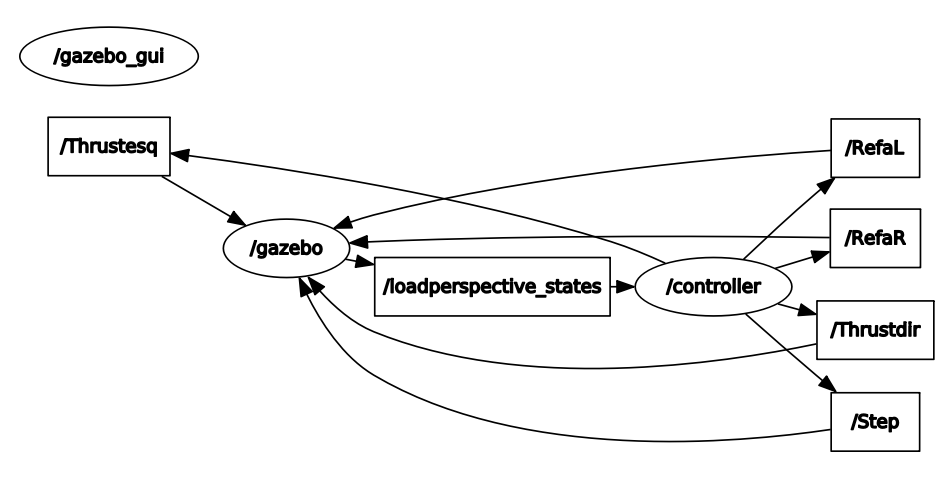
\includegraphics[width=350pt]{figuras/v2loadgraph.png}
	\caption{UAV 2.0 Load Communication}
	\label{v2loadgraph}
\end{figure*}


\subsection{UAV 3.0}

In the UAV 3.0 project aerodynamic surfaces were added . By doing so, a small deflexion in a aerodynamic surface can generate aerodynamic forces that can improve cruise flight. Similar to UAV 2.0, the UAV 3.0 was used for several works developed in the ProVANT project as can be shown in the paper: \url{https://www.researchgate.net/publication/311919640_A_robust_adaptive_mixing_control_for_improved_forward_flight_of_a_tilt-rotor_UAV}



\begin{figure*}[!ht]
	\centering
	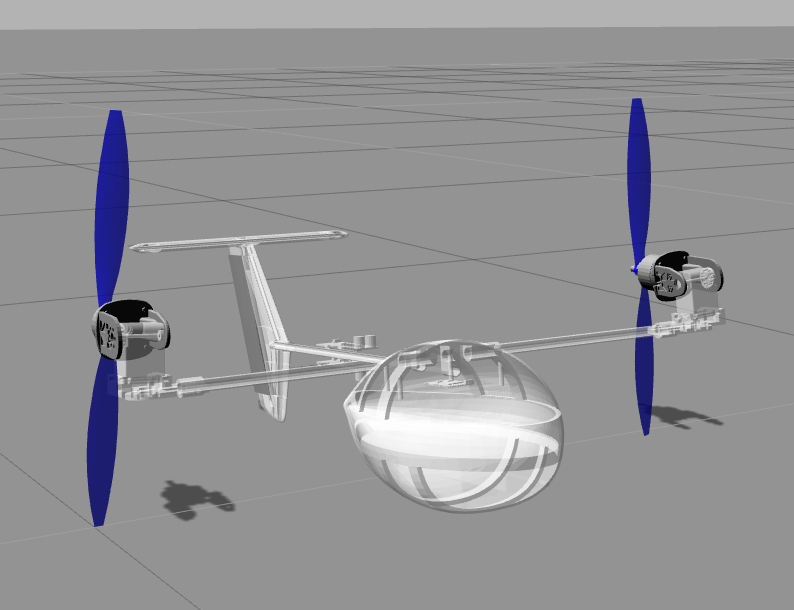
\includegraphics[width=250pt]{figuras/vant3.png}
	\caption{UAV 3.0}
	\label{vant3}
\end{figure*}

The kinematic and dynamic model were developed using the coordinate frames showned in figure \ref{v3frames} and the parameters in table \ref{v3tab}

\begin{figure} [!ht]
	\centering
	\begin{minipage}{.5\textwidth}
		\centering
		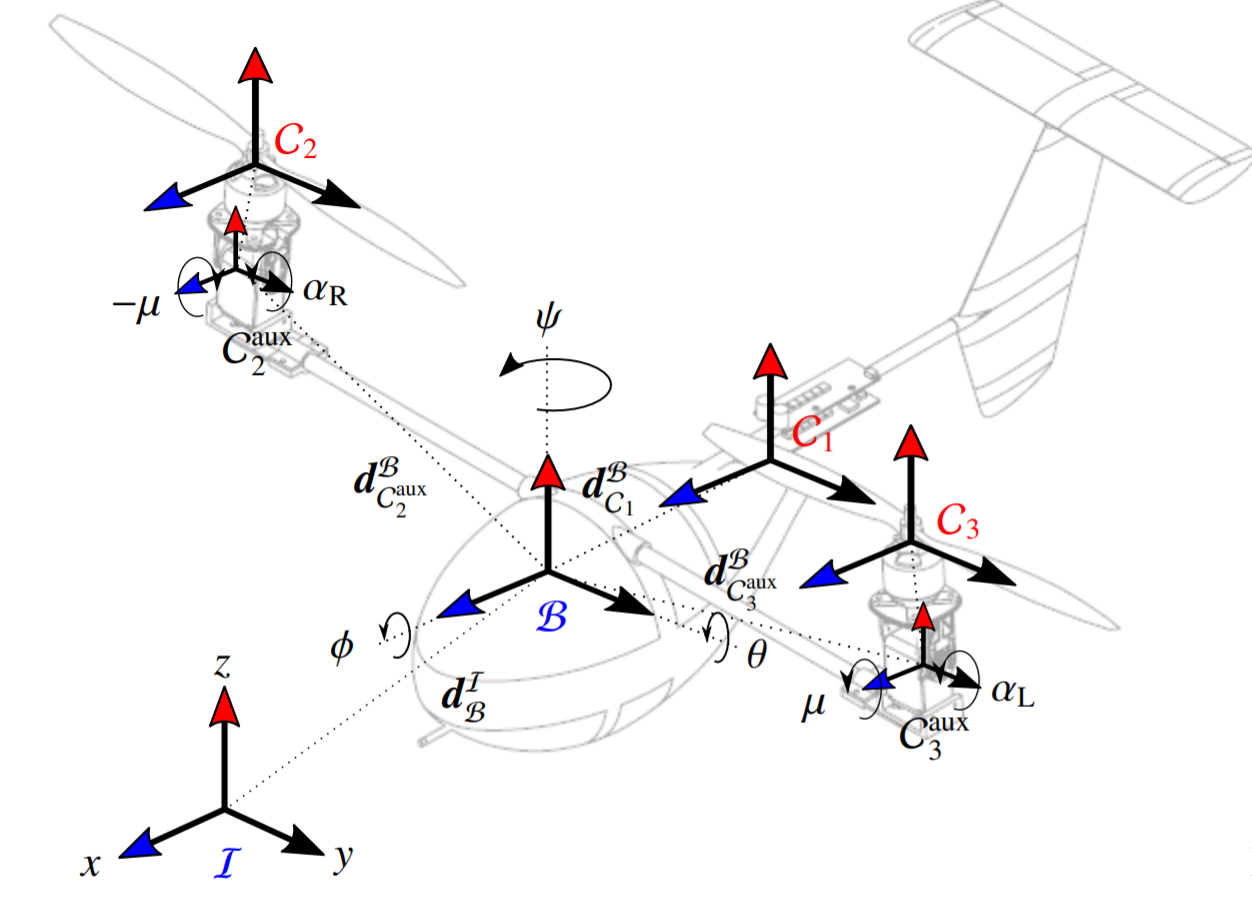
\includegraphics[width=250pt]{figuras/v3frames}
		\caption{UAV 3.0 Coordinate Frames}
		\label{v3frames}
	\end{minipage}%
	\begin{minipage}{.5\textwidth}
		\centering
		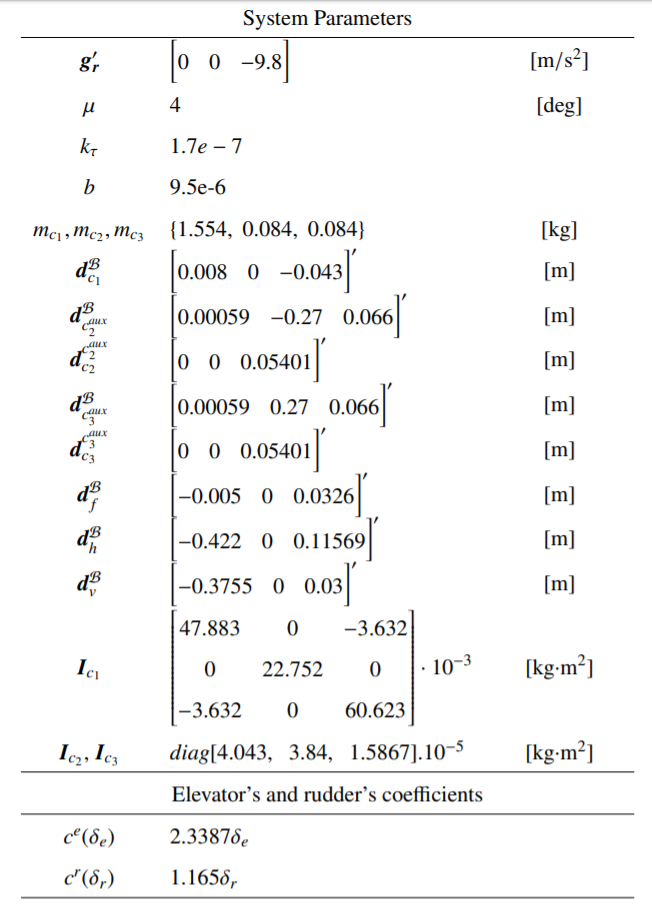
\includegraphics[width=250pt]{figuras/v3tab}
		\caption{UAV 3.0 Parameters.}
		\label{v3tab}
	\end{minipage}
\end{figure}

The control strategy for UAV 3.0 is a $\frac{\mathcal{H}_2}{\mathcal{H_\infty}}$ with the following state vector:
\begin{equation*}
\bm{X} = \begin{bmatrix}
u \\
v \\
w \\
p \\
q \\
r\\
\dot\alpha_R \\
\dot\alpha_L \\
z \\
\phi \\
\theta \\
\psi \\
\alpha_R \\
\alpha_L \\
\int{u} \\
\int{v} \\
\int{\psi} \\         
\end{bmatrix}
\end{equation*} 

Where, $(u,v,w)$ are the linear velocities of the \textit{UAV body frame} with respect to the \textit{inertial frame} expressed in the \textit{UAV body frame}, and ($p,q,r$) are the angular velocities of the \textit{UAV body frame} with respect to the \textit{inertial frame} expressed in the \textit{UAV body frame}.

Three plugins were used for the UAV 3.0 simulation: The "aerodinamica" plugin that applies the force generated by the propellers and controls the aerodynamic forces, the "servo" plugin to actuate de servo motors, and the "statespace" plugin to access the UAV state vector needed for control. This plugins are further detailed in appendix \ref{pluginsAp}. In figure \ref{v3graph}, the rectangular shapes indicate the ros topics and the roud shapes represent the ros nodes trigger in the simulation.
 


\begin{figure*}[!ht]
	\centering
	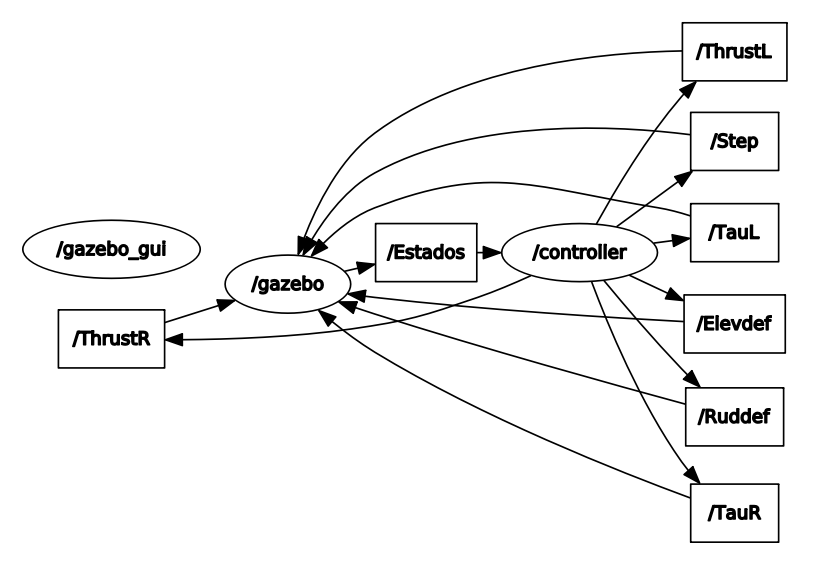
\includegraphics[width=350pt]{figuras/v3graph.png}
	\caption{UAV 3.0 Communication}
	\label{v3graph}
\end{figure*}


\subsection{UAV 4.0}

The UAV 4.0 was developed in a partnership between the Federal University of Minas Gerais, Federal University of Santa Catarina and the University of Seville with the goal to develop a fast response UAV for search and rescue missions.


\begin{figure*}[!ht]
	\centering
	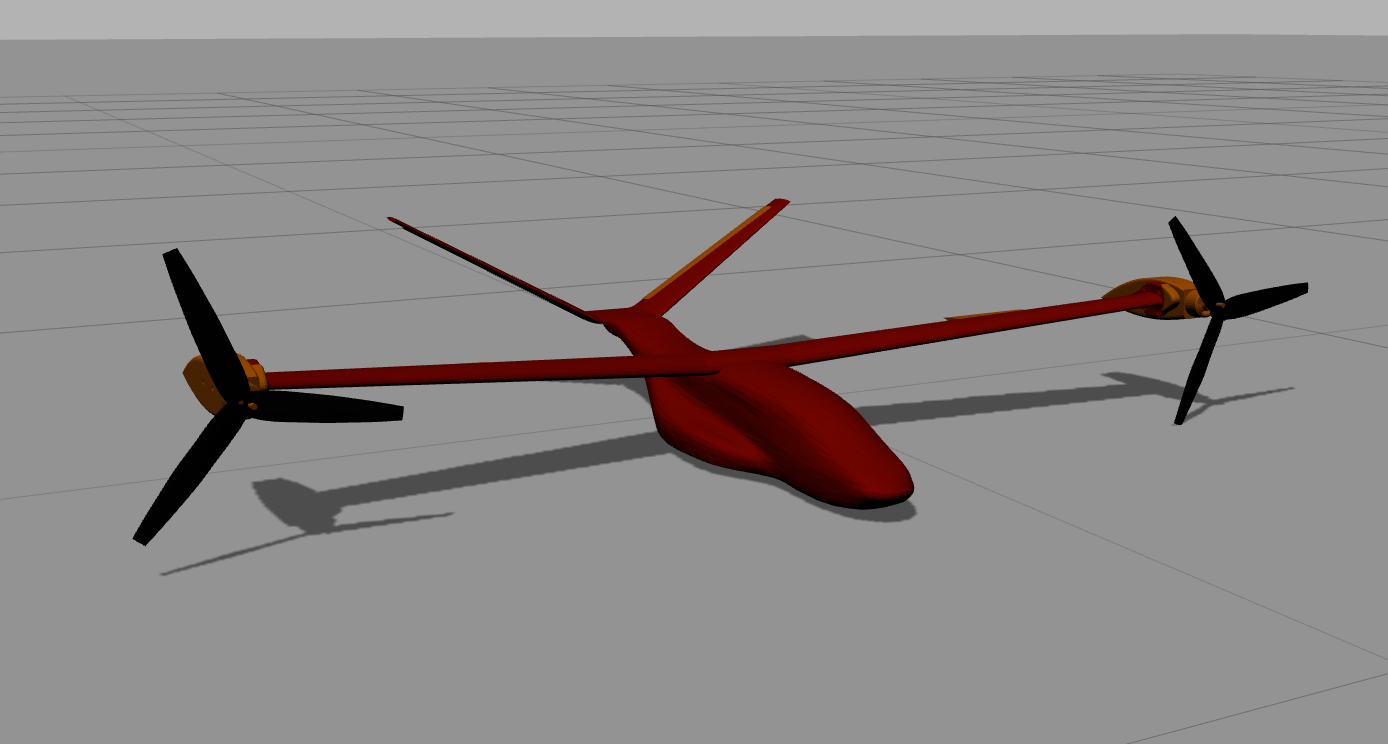
\includegraphics[width=250pt]{figuras/vant4.png}
	\caption{VANT 4.0}
	\label{vant4}
\end{figure*}


The kinematic and dynamic model were developed using the coordinate frames showned in figure \ref{v4frames} and the parameters in table \ref{v4tab}. More on the kinematic and dynamic models of UAV 4.0: \url{https://www.researchgate.net/publication/337571676_Modelagem_e_Simulacao_de_um_VANT_Convertivel_Tilt-rotor}

\begin{figure} [!ht]
	\centering
	\begin{minipage}{.5\textwidth}
		\centering
		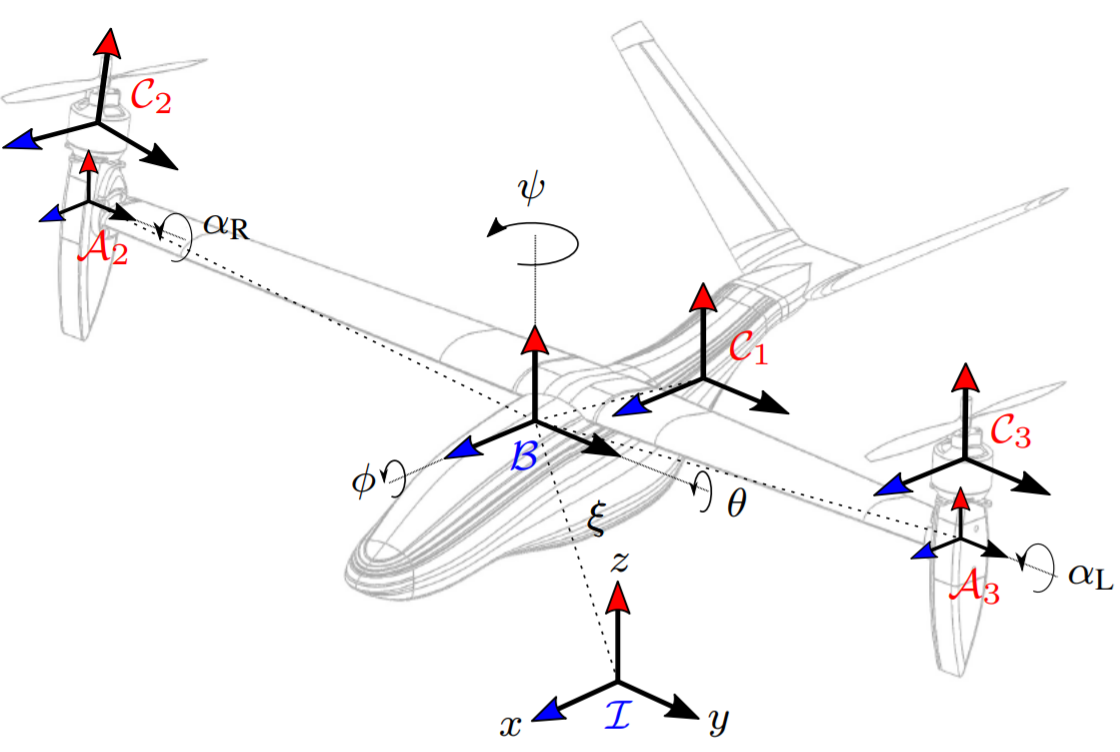
\includegraphics[width=250pt]{figuras/v4frames}
		\caption{UAV 4.0 Coordinate Frames.}
		\label{v4frames}
	\end{minipage}%
	\begin{minipage}{.5\textwidth}
		\centering
		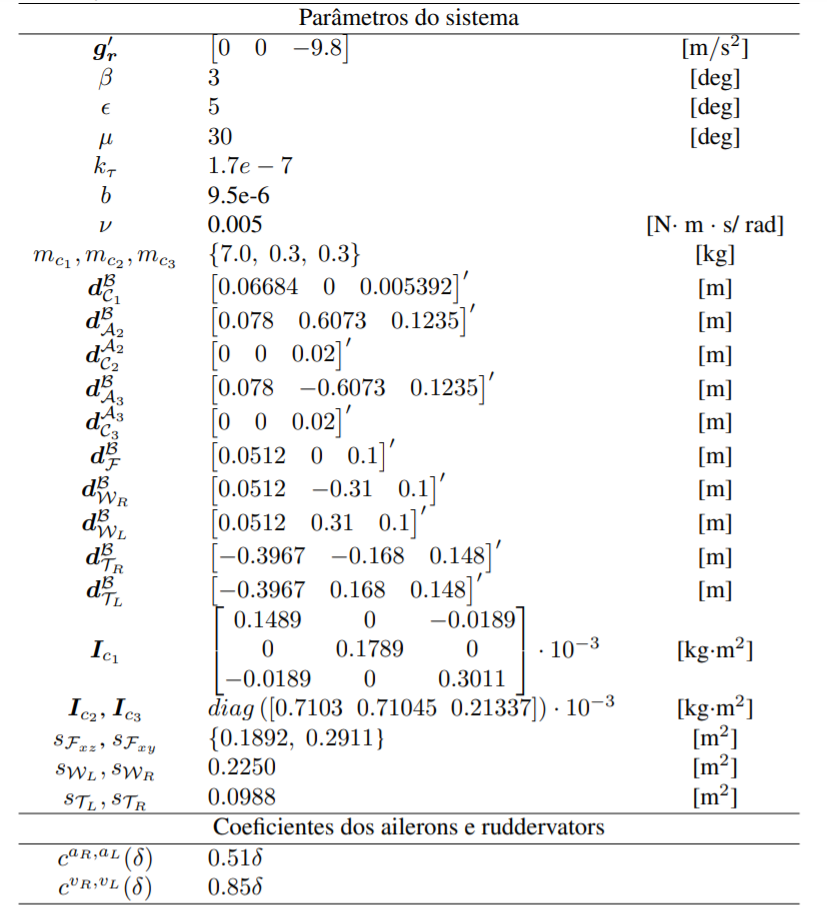
\includegraphics[width=250pt]{figuras/v4tab}
		\caption{UAV 4.0 Parameters.}
		\label{v4tab}
	\end{minipage}
\end{figure}

The control strategy for UAV 3.0 is a $\mathcal{W}_\infty$ with the following state vector:

\begin{equation*}
\bm{X} = \begin{bmatrix}
\dot{\bm{q_{s}}}' & \dot{\tilde{\bm{q_{c}}}}' & \tilde{\bm{q_{c}}}' & \int_{0}^{t}{\tilde{\bm{q_{c}}}'}dt
\end{bmatrix}'
\end{equation*}

Where, $\bm{q_{s}}$ are the stabilized degrees of freedom, $\bm{q_{c}}$ are the controled degrees of freedom, and $\tilde{\bm{q_{c}}} \coloneqq  \bm{q_{c}} - \bm{q_{c_{r}}}$ where $\bm{q_{c_{r}}}$ are the desired values of $\bm{q_{c}}$. Aside:
\begin{equation*}
\bm{q_{s}} = \begin{bmatrix}
\alpha_R & \alpha_L & \phi & \theta
\end{bmatrix}'
\end{equation*}
and
\begin{equation*}
\bm{q_{c}} = \begin{bmatrix}
\psi & x & y & z
\end{bmatrix}'
\end{equation*}

To simulate the UAV 4.0 six plugins are required: the "Aerodinâmica4dot0" plugin implements the aerodynamic forces, the "statespace" plugin to access the UAV state vector needed for control, the "servo" plugin to actuate the \textit{ailerons}, \textit{rudders} and rotors, the "PathPlotter" plugin to visualize the performed trajectory in Rviz, "VisualPropellers" to visualize the propellers movement, and "DataSaveTiltRotor" to save data in ".txt" files at the \textit{Matlab} directory.This plugins are further detailed in appendix \ref{pluginsAp}. In figure \ref{v4graph}, the rectangular shapes indicate the ros topics and the roud shapes represent the ros nodes trigger in the simulation.


\begin{figure*}[!ht]
	\centering
	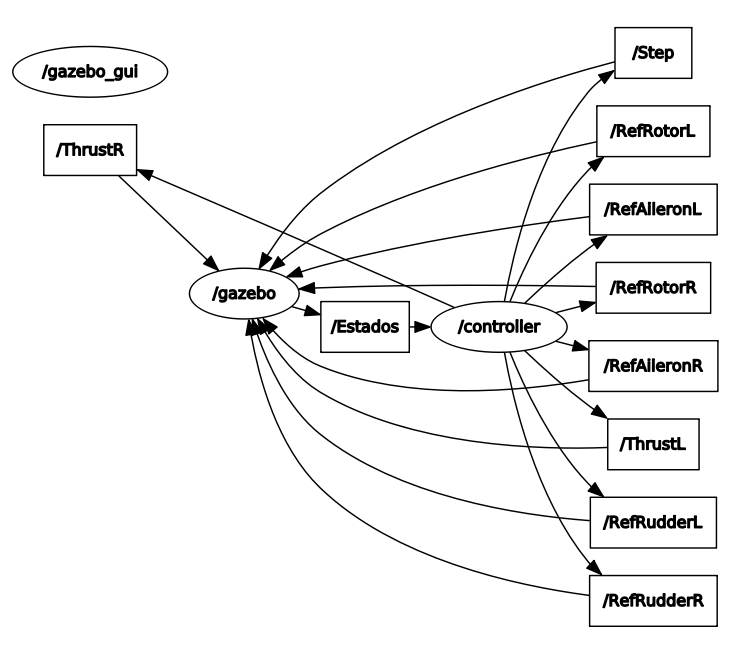
\includegraphics[width=350pt]{figuras/v4graph.png}
	\caption{UAV 4.0 Communication}
	\label{v4graph}
\end{figure*}





\subsection{Quadrotor}

The Quadrotor study field in the UAV literature is a productive field for research. To take advantage of that fact, a UAV of type Quadrotor was implemented in the simulator.


\begin{figure*}[!ht]
	\centering
	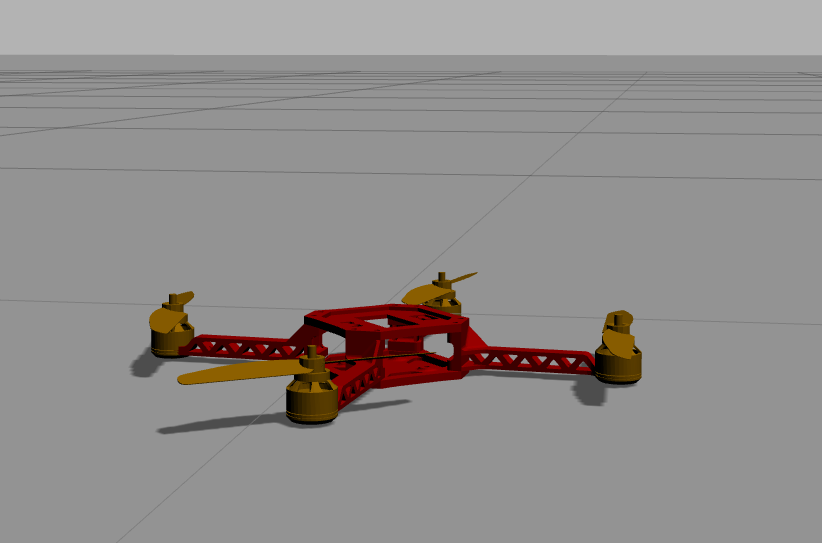
\includegraphics[width=250pt]{figuras/quad.png}
	\caption{Quadrotor}
	\label{quad}
\end{figure*}


The kinematic and dynamic model were developed using the coordinate frames showned in figure \ref{quadframes} and the parameters in table \ref{quadtab}

\begin{figure} [!ht]
	\centering
	\begin{minipage}{.5\textwidth}
		\centering
		\includegraphics[width=250pt]{figuras/quadframes}
		\caption{Quadrotor Coordinate Frames.}
		\label{quadframes}
	\end{minipage}%
	\begin{minipage}{.5\textwidth}
		\centering
		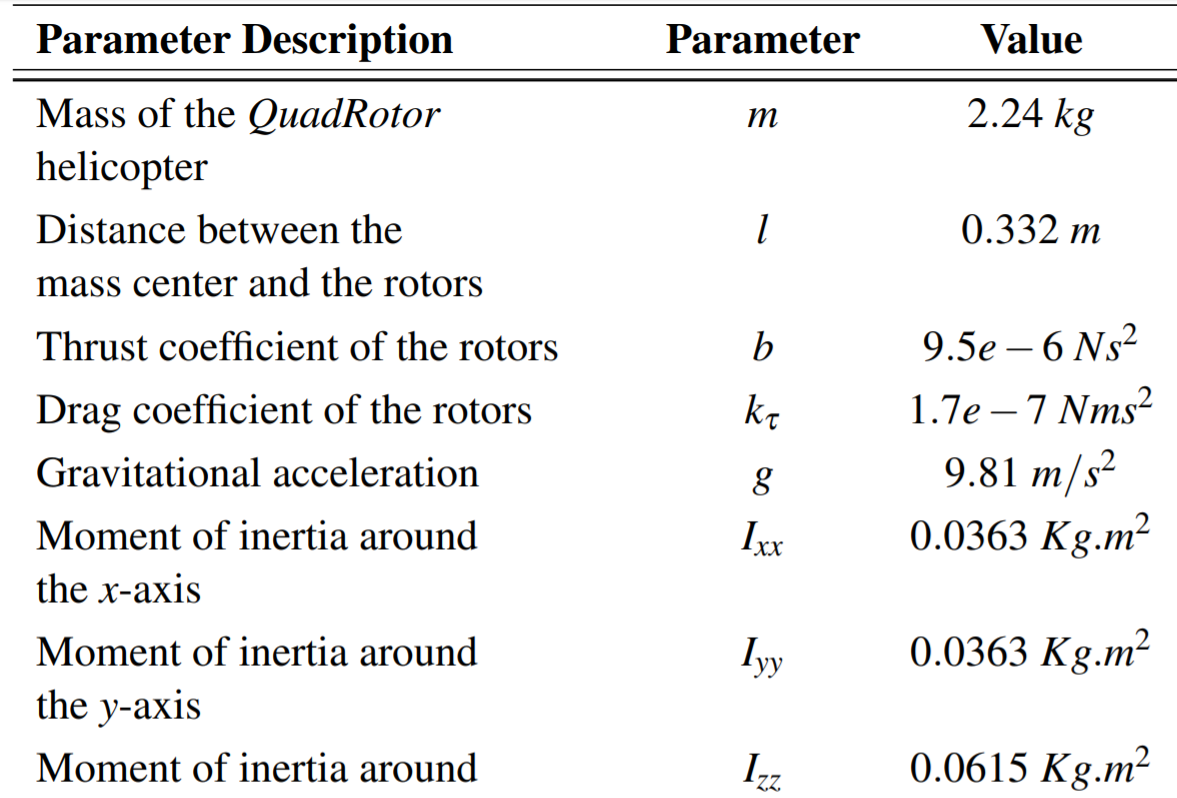
\includegraphics[width=250pt]{figuras/quad_parameters_table}
		\caption{Quadrotor Parameters.}
		\label{quadtab}
	\end{minipage}
\end{figure}

The Quadrotor was implemented with an LQR control strategy with the following state vector:
\begin{equation*}
\bm{X} = \begin{bmatrix}
\bm{q} & \dot{\bm{q}}
\end{bmatrix}'
\end{equation*}

Onde, 
\begin{equation*}
\bm{q} = \begin{bmatrix}
x & y & z & \phi & \theta & \psi
\end{bmatrix}'
\end{equation*}


To simulate the Quadrotor four plugins are used: "QuadForces" to implement the forces on the four motors, "QuadData" to obtain the state vector needed for control, "PathPlotter" to visualize the Quadrotor trajectory on rviz, "VisualPropellers" to visualize the propellers movement. This plugins are further detailed in appendix \ref{pluginsAp}. In figure \ref{quadgraph}, the rectangular shapes indicate the ros topics and the roud shapes represent the ros nodes trigger in the simulation.


\begin{figure*}[!ht]
	\centering
	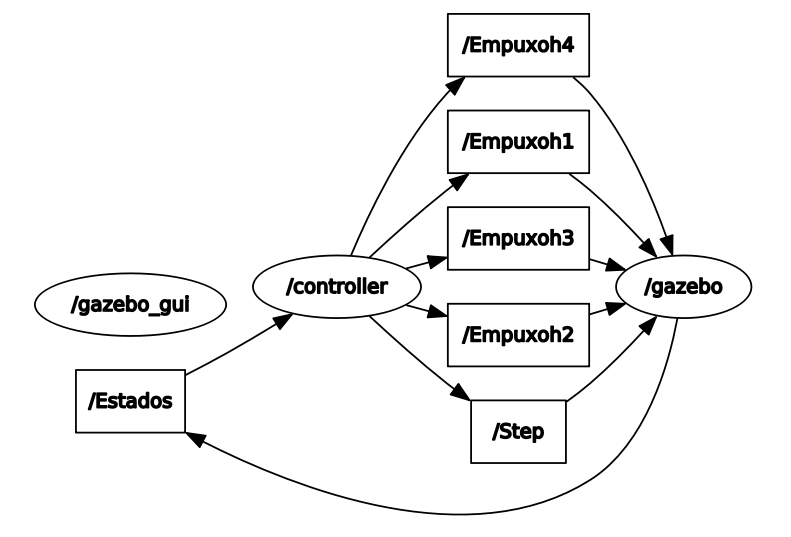
\includegraphics[width=350pt]{figuras/quadgraph.png}
	\caption{Quadrotor Comunication.}
	\label{quadgraph}
\end{figure*}
